
%(BEGIN_QUESTION)
% Copyright 2009, Tony R. Kuphaldt, released under the Creative Commons Attribution License (v 1.0)
% This means you may do almost anything with this work of mine, so long as you give me proper credit

\vbox{\hrule \hbox{\strut \vrule{} {\bf Desktop Process exercise} \vrule} \hrule}

PID (Proportional-Integral-Derivative) closed-loop control is a perplexing subject to master, without a doubt.  An essential component of any course of study in PID control is adequate experimental time spent operating and tuning real PID-controlled processes.  In this course, one of the ways you will gain hands-on experience with PID control is to operate a miniature process that easily fits on a desktop.

A simple diagram of this ``Desktop Process'' is shown here, where a single-loop controller controls the speed of a DC electric motor:

$$\includegraphics[width=15.5cm]{i04257x02.eps}$$

The motor receives its power from the Variable-Speed Drive (VSD), and reports shaft speed to the controller by means of a tachogenerator (``tach'') which generates a DC voltage proportional to shaft speed.

\vskip 10pt

Determine the necessary action of the loop controller ({\it direct} or {\it reverse}), assuming that a greater current signal sent to the motor drive causes the motor to spin faster.

%Multiple options exist for such a ``Desktop Process,'' but one that is relatively easy to build and operate is where a PID controller controls the speed of a DC electric motor, which then controls the temperature of a soldering iron tip (or alternatively, controls the temperature down-wind of a soldering iron tip):

%$$\includegraphics[width=15.5cm]{i04257x01.eps}$$

%You will build such a Desktop Process in stages, beginning with the motor speed control, and eventually working up to a ``cascade'' control system where the fan's speed controls temperature.

\vskip 20pt \vbox{\hrule \hbox{\strut \vrule{} {\bf Suggestions for Socratic discussion} \vrule} \hrule}

\begin{itemize}
\item{} If you do not have access to a Desktop Process, you may gain valuable experience tuning PID loops by using computer simulation software.  Try searching the internet for free PID simulation programs, or web-based simulations you can run using a web browser.  A popular (and free!) PID simulator program is made by {\it Dex Automation}.
\end{itemize}

\underbar{file i04257}
%(END_QUESTION)





%(BEGIN_ANSWER)


%(END_ANSWER)





%(BEGIN_NOTES)

\vfil \eject

\noindent
{\bf Prep Quiz:}

The ``Desktop Process'' described in the worksheet uses what sort of process to provide practice with PID tuning?

\begin{itemize}
\item{} Light (brightness) control
\vskip 5pt 
\item{} Water level control
\vskip 5pt 
\item{} Temperature control
\vskip 5pt 
\item{} Water flow control
\vskip 5pt 
\item{} Motor speed control
\vskip 5pt 
\item{} Air pressure control
\end{itemize}


%INDEX% Desktop Process: introduction 

%(END_NOTES)


